\section{Thrust 3. Voice-Driven Features for an IDE to support VIPLs}
\label{sec:thrust3}

%\begin{figure}[t]
%\centering
%\begin{minipage}{.48\textwidth}
%\centering
%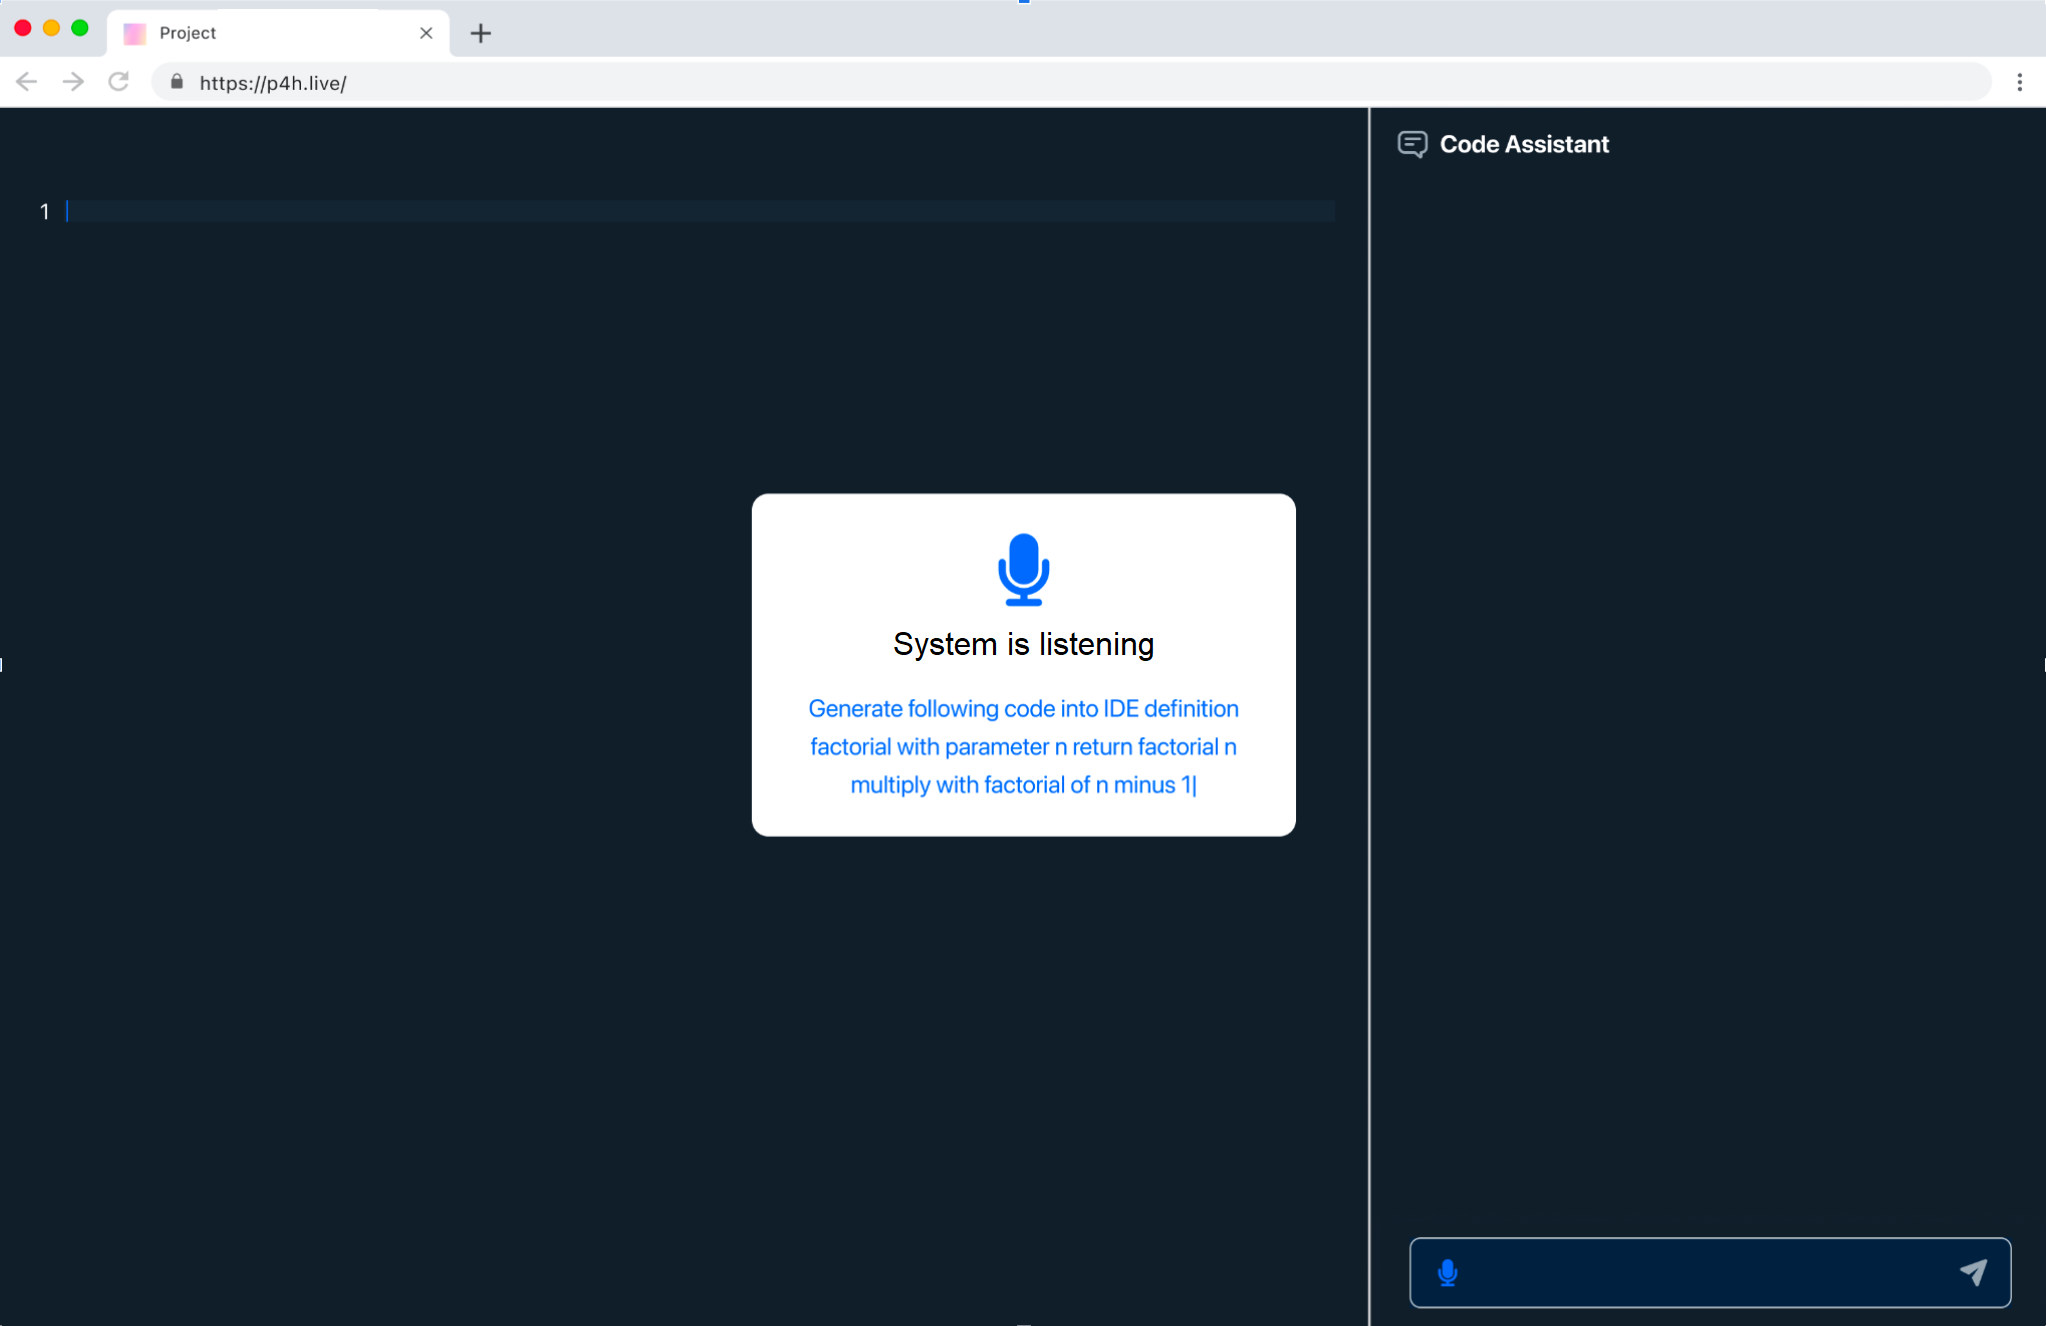
\includegraphics[width=.98\textwidth]{p4h-1}
%\end{minipage}
%\begin{minipage}{.48\textwidth}
%\centering
%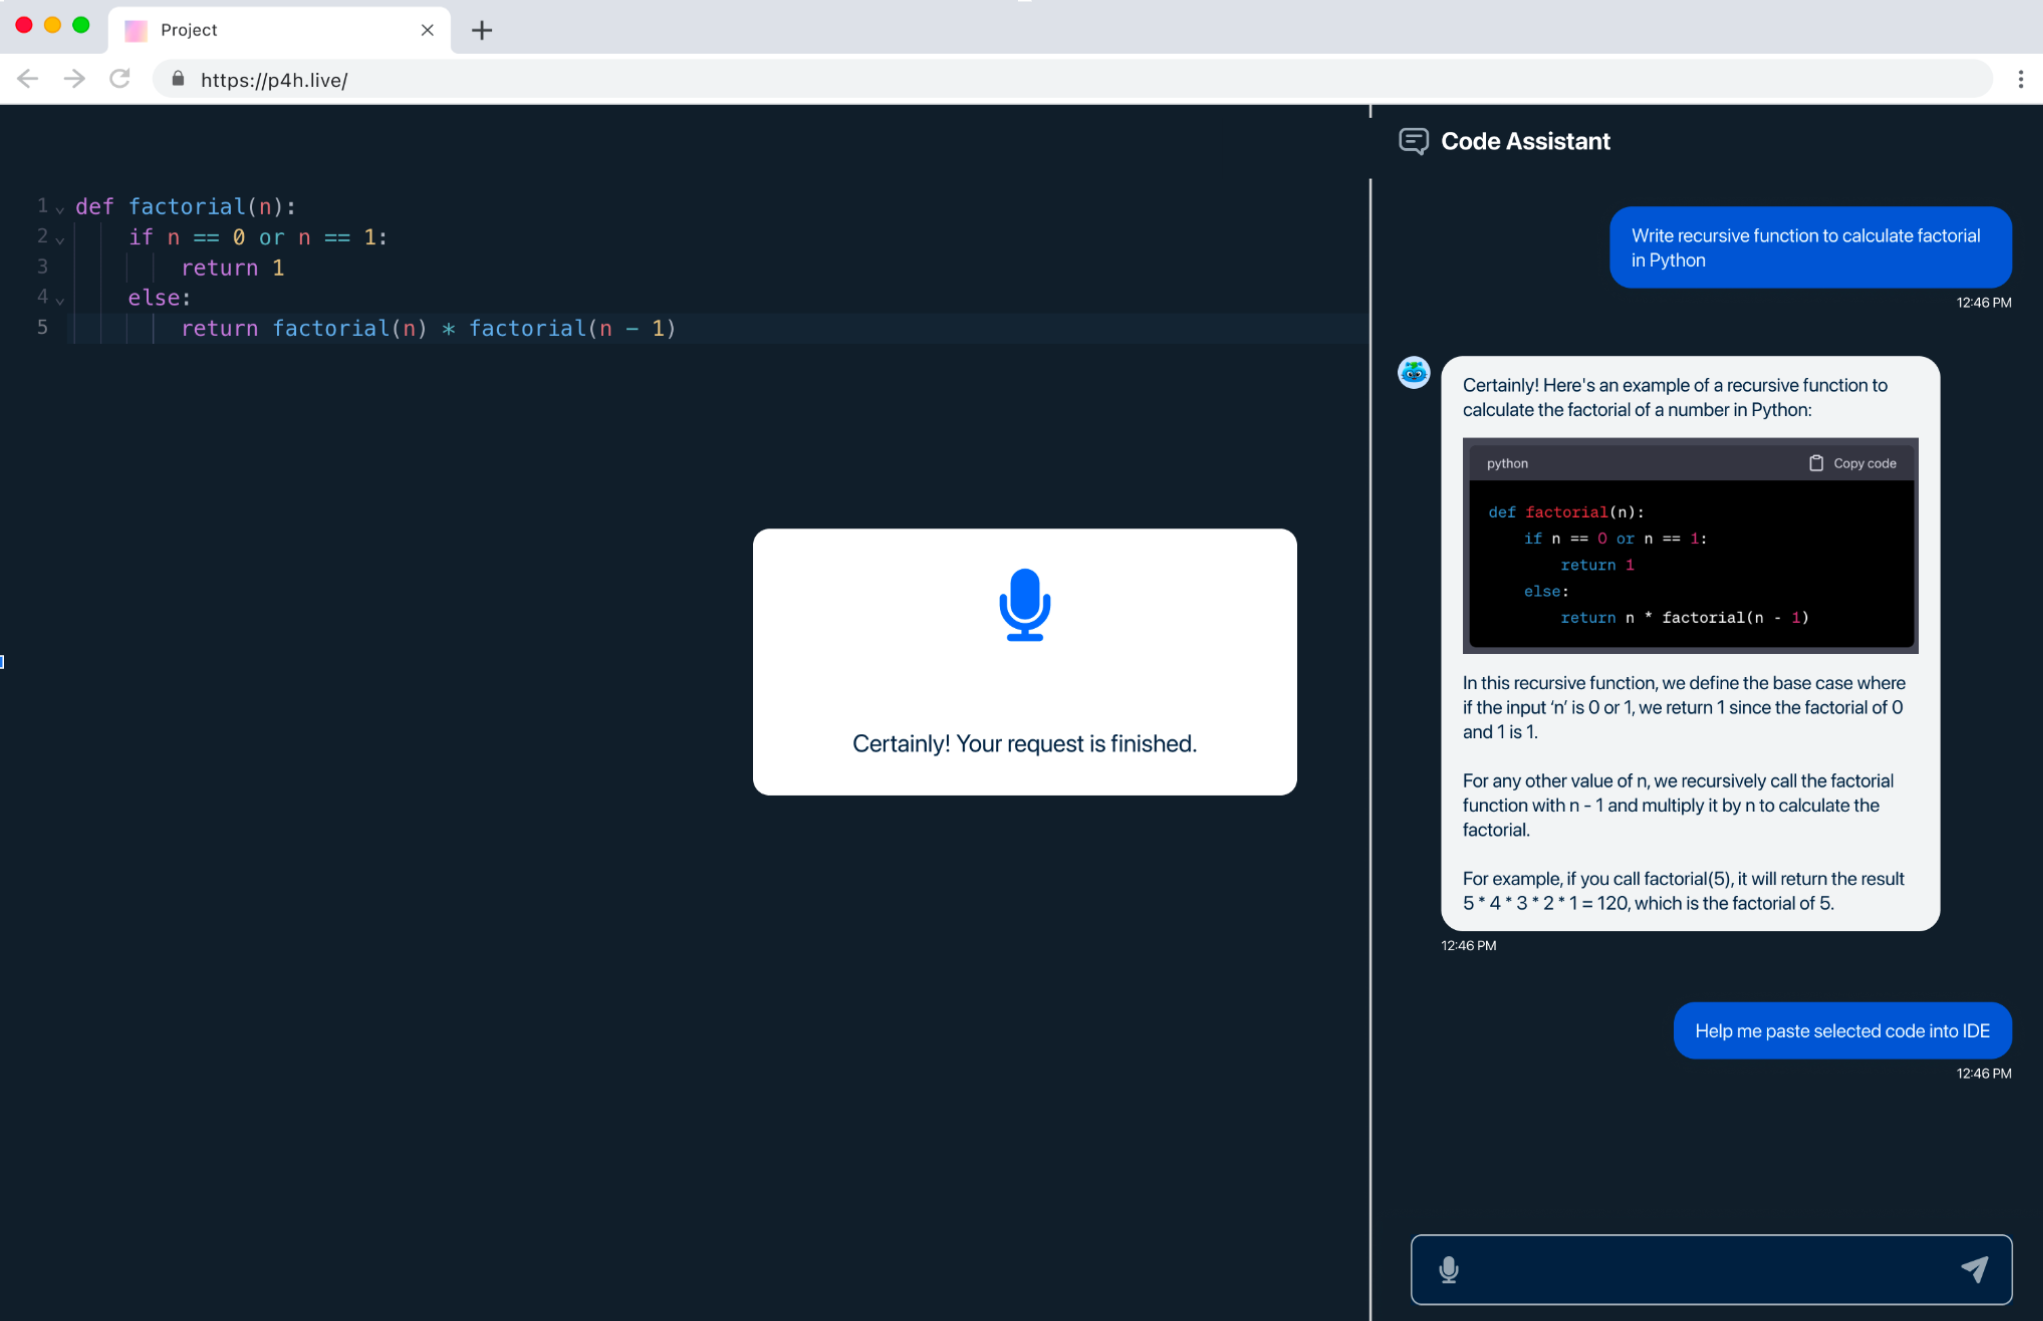
\includegraphics[width=.98\textwidth]{p4h-2}
%\end{minipage}  
%\caption{Voice to Code Generation}
%\label{thrust3-one}
%\end{figure}

\begin{figure}[t]
\centering
\begin{minipage}{.48\textwidth}
%\begin{figure}[t]
\centering
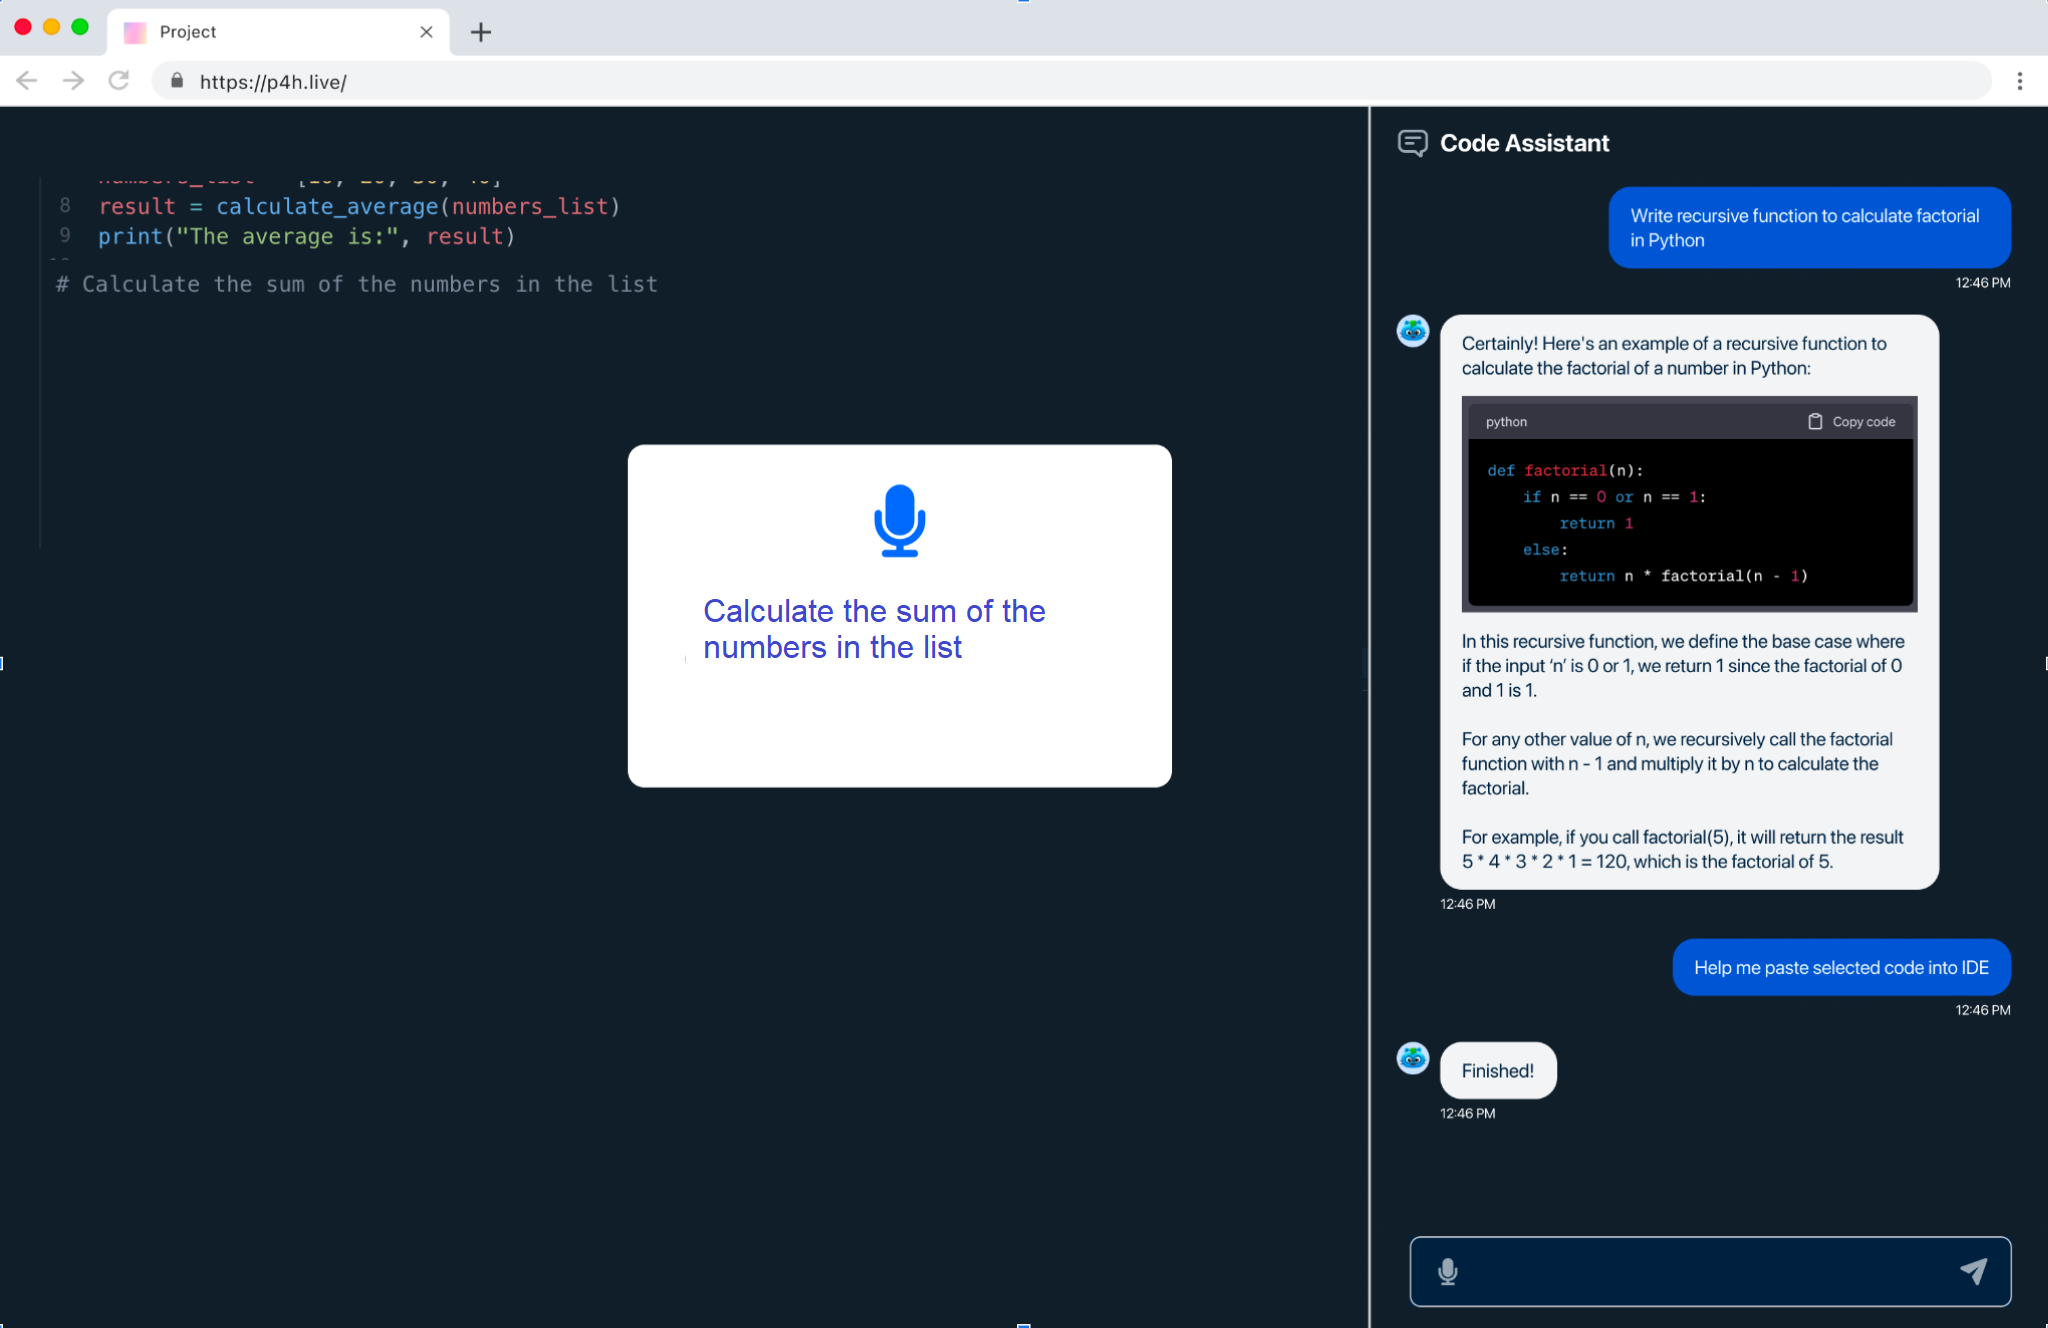
\includegraphics[width=.98\textwidth]{p4h-3}
%\caption{caption 1}
%\label{fig:left}
%\end{figure}
\end{minipage}
\begin{minipage}{.48\textwidth}
%\begin{figure}[t]
\centering
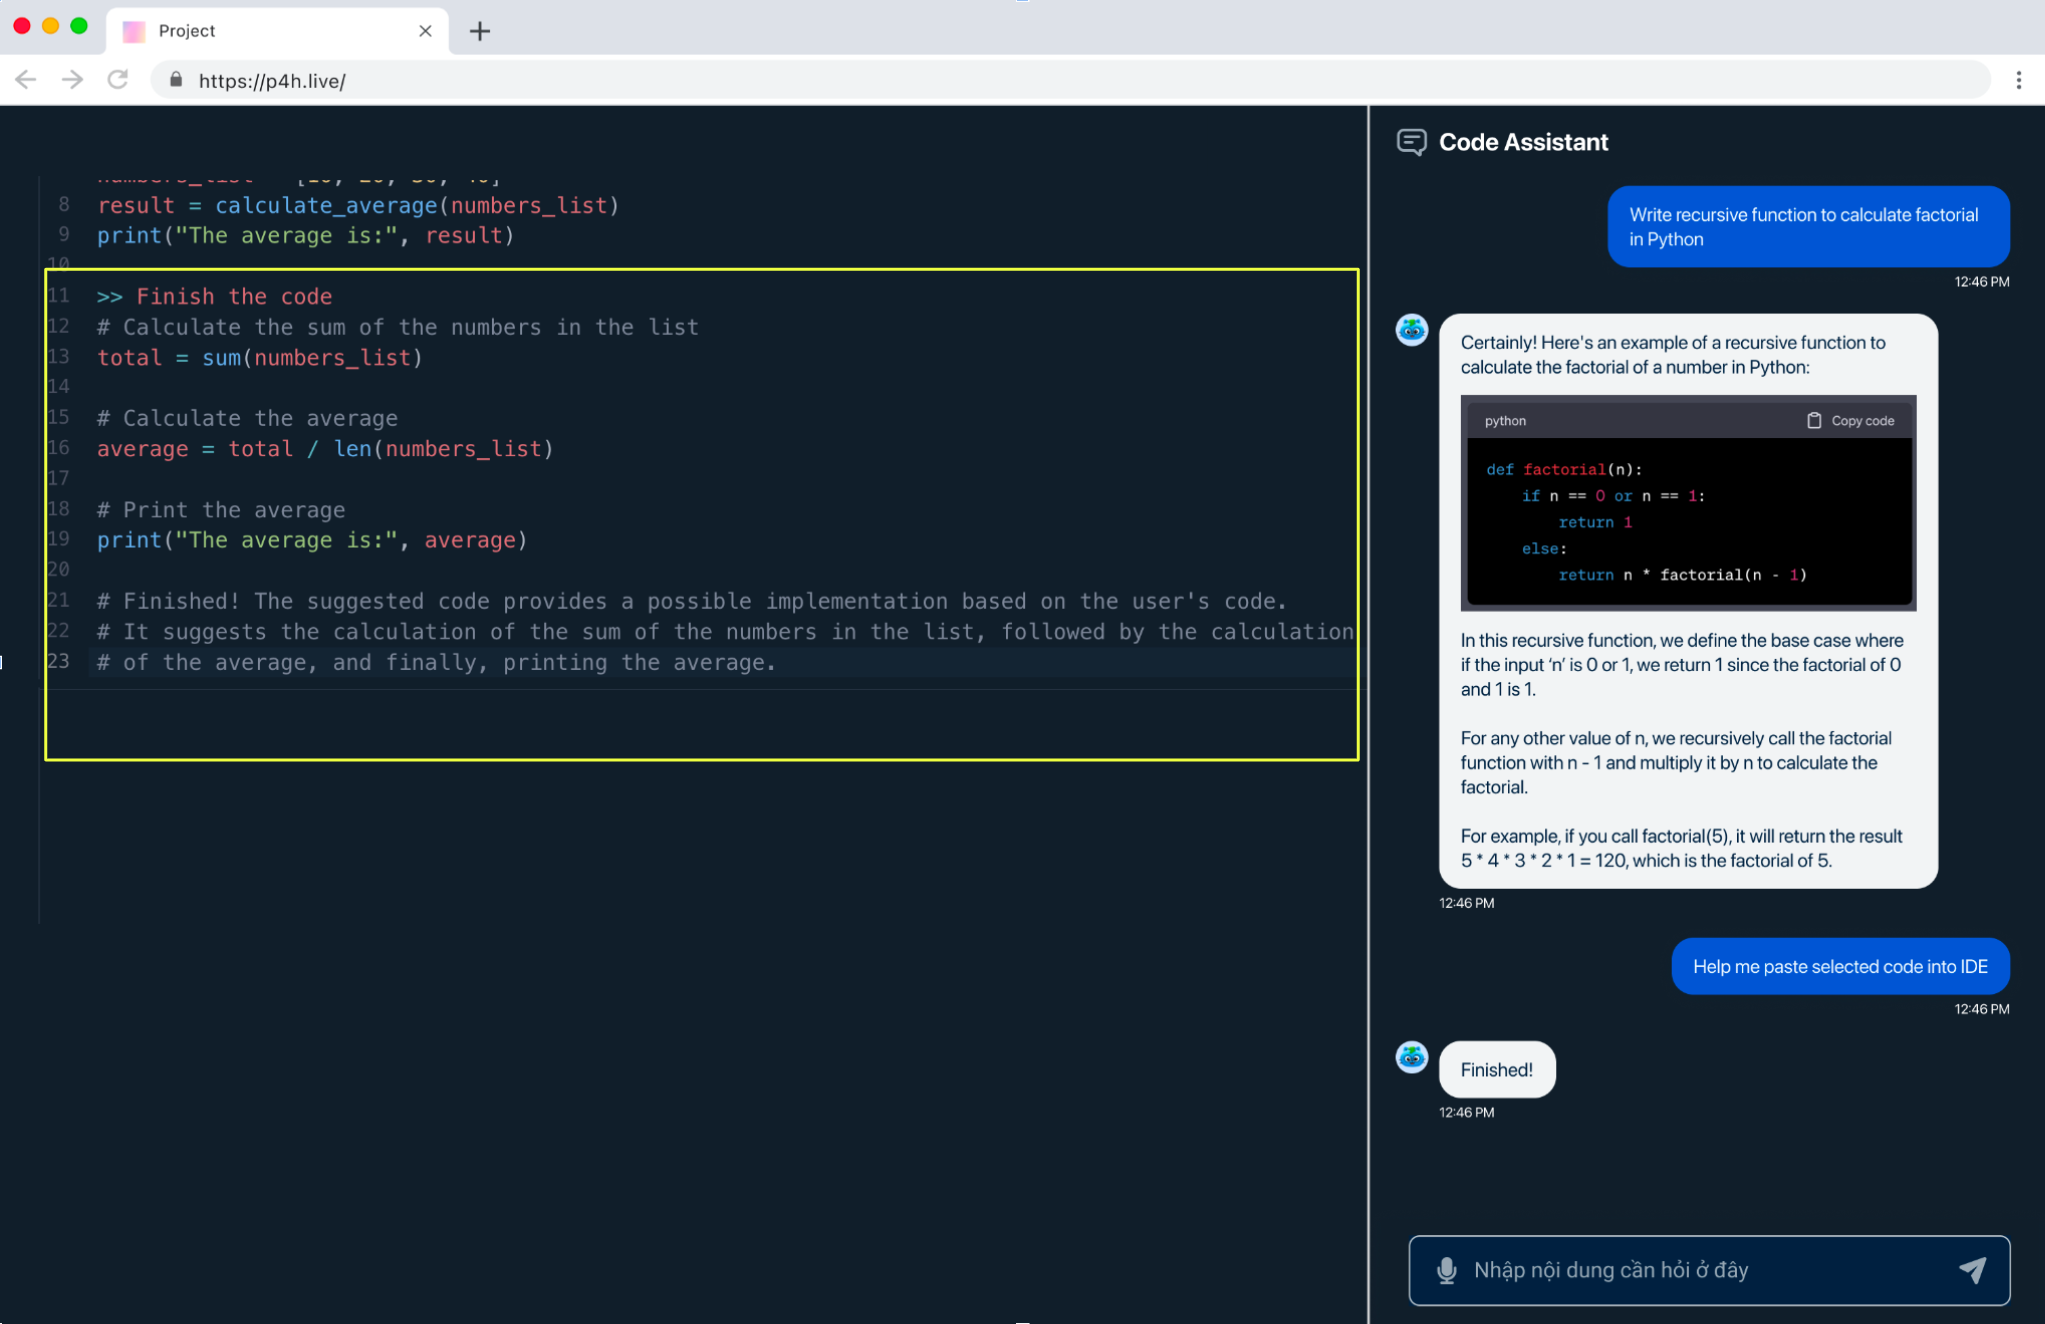
\includegraphics[width=.98\textwidth]{p4h-4}
%\caption{caption 2}
%\label{fig:right}
%\end{figure}
\end{minipage}  
%\vspace{-18pt}
\caption{In-line Voice to Code Generation}
\label{thrust3-one}
\end{figure}

{\bf Voice to Code Generation for Adaptive Learning.} In this use case
scenario (Figure~\ref{thrust3-one}), let's explore how a VIPL
interacts with our proposed environment to create
source code for calculating the factorial of a number. This scenario
showcases the environment's voice interaction and code generation
capabilities.

{\em Initialization}: The visually-impaired programmer initiates the
programming environment by saying, "Hey, Environment, start a new code
project for calculating factorial."

{\em Voice Interaction}: The environment responds with a synthesized voice,
"Sure, please specify the number for which you want to calculate the
factorial." The programmer responds, "Calculate the factorial of 5."

{\em Code Generation}: The programming environment interprets the user's
request and generates the code snippet using advanced voice
recognition and generative AI technologies.  The environment then
communicates, "I've generated the code to calculate the factorial of
5. Here's the code for you:".

{\em Verification}: The generated code is read back to the user through synthesized speech, and the user can confirm its accuracy.
The user says, "Please read back the generated code."

{\em Confirmation}: The environment reads the code aloud, "Def factorial(n): If n equals 0, return 1. Else, return n times factorial(n minus 1). Result equals factorial(5). Print 'The factorial of 5 is:' and the result." The user confirms that the code accurately reflects their intent.

{\em Execution}: The programmer can proceed to execute the code by saying, "Execute the code." The environment executes the code, and the synthesized speech reads the result, "The factorial of 5 is: 120."

{\em Documentation}: The programmer can further enhance the code by documenting it using voice commands. For example, they can say, "Add a comment: This code calculates the factorial of a number."

{\em Integration}: If the programmer has an existing project, they can
integrate this code seamlessly into their project using voice
commands, ensuring a cohesive workflow.

%=========================================================

%\begin{figure}[t]
%\centering
%\begin{minipage}{.48\textwidth}
%\centering
%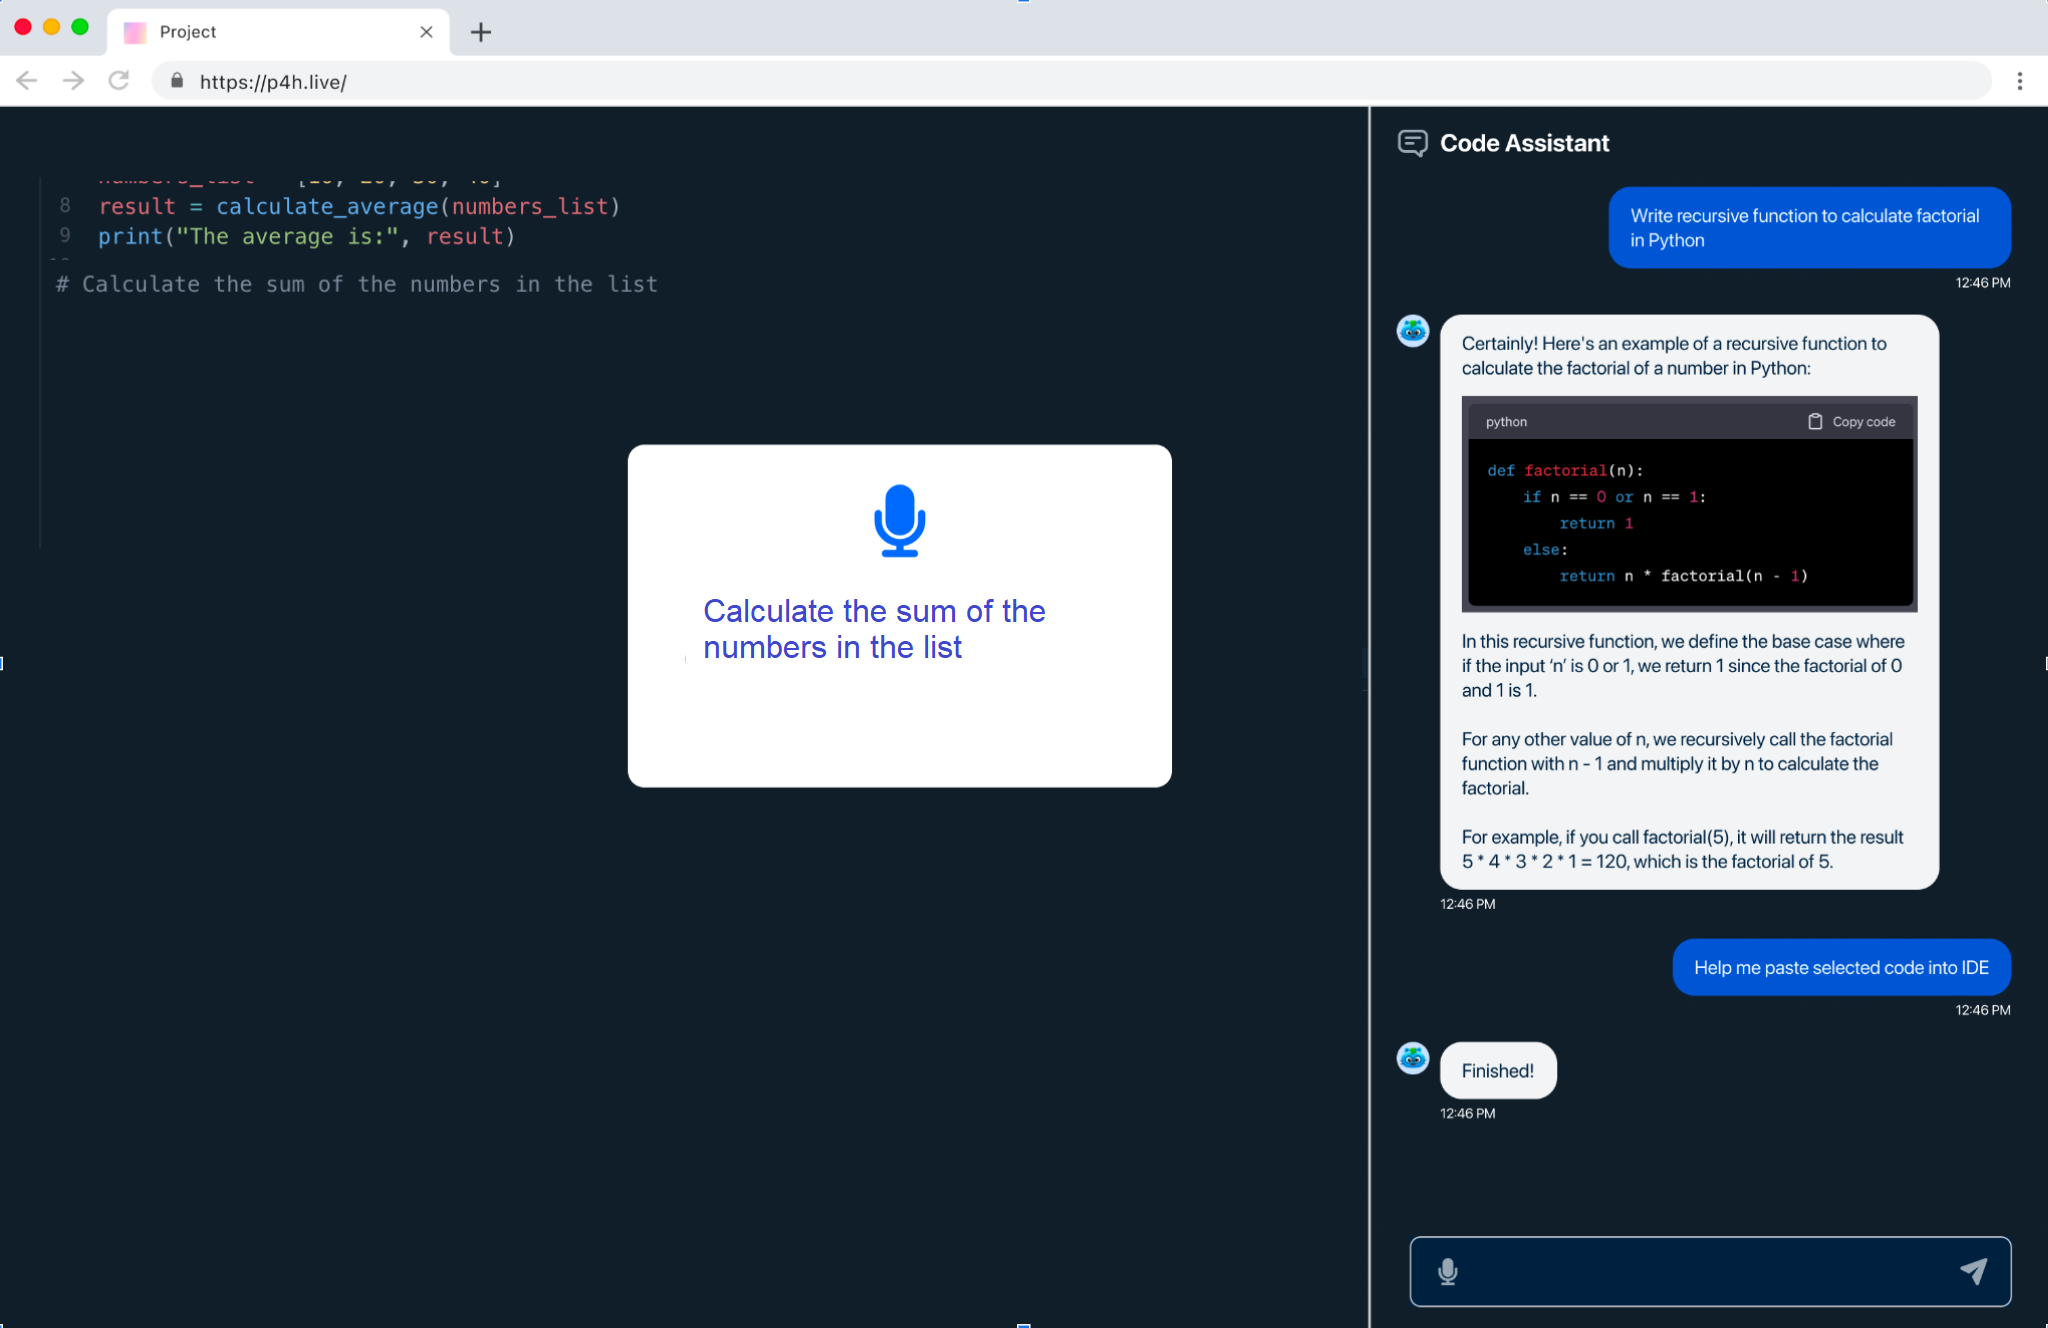
\includegraphics[width=.98\textwidth]{p4h-3}
%\end{minipage}
%\begin{minipage}{.48\textwidth}
%\centering
%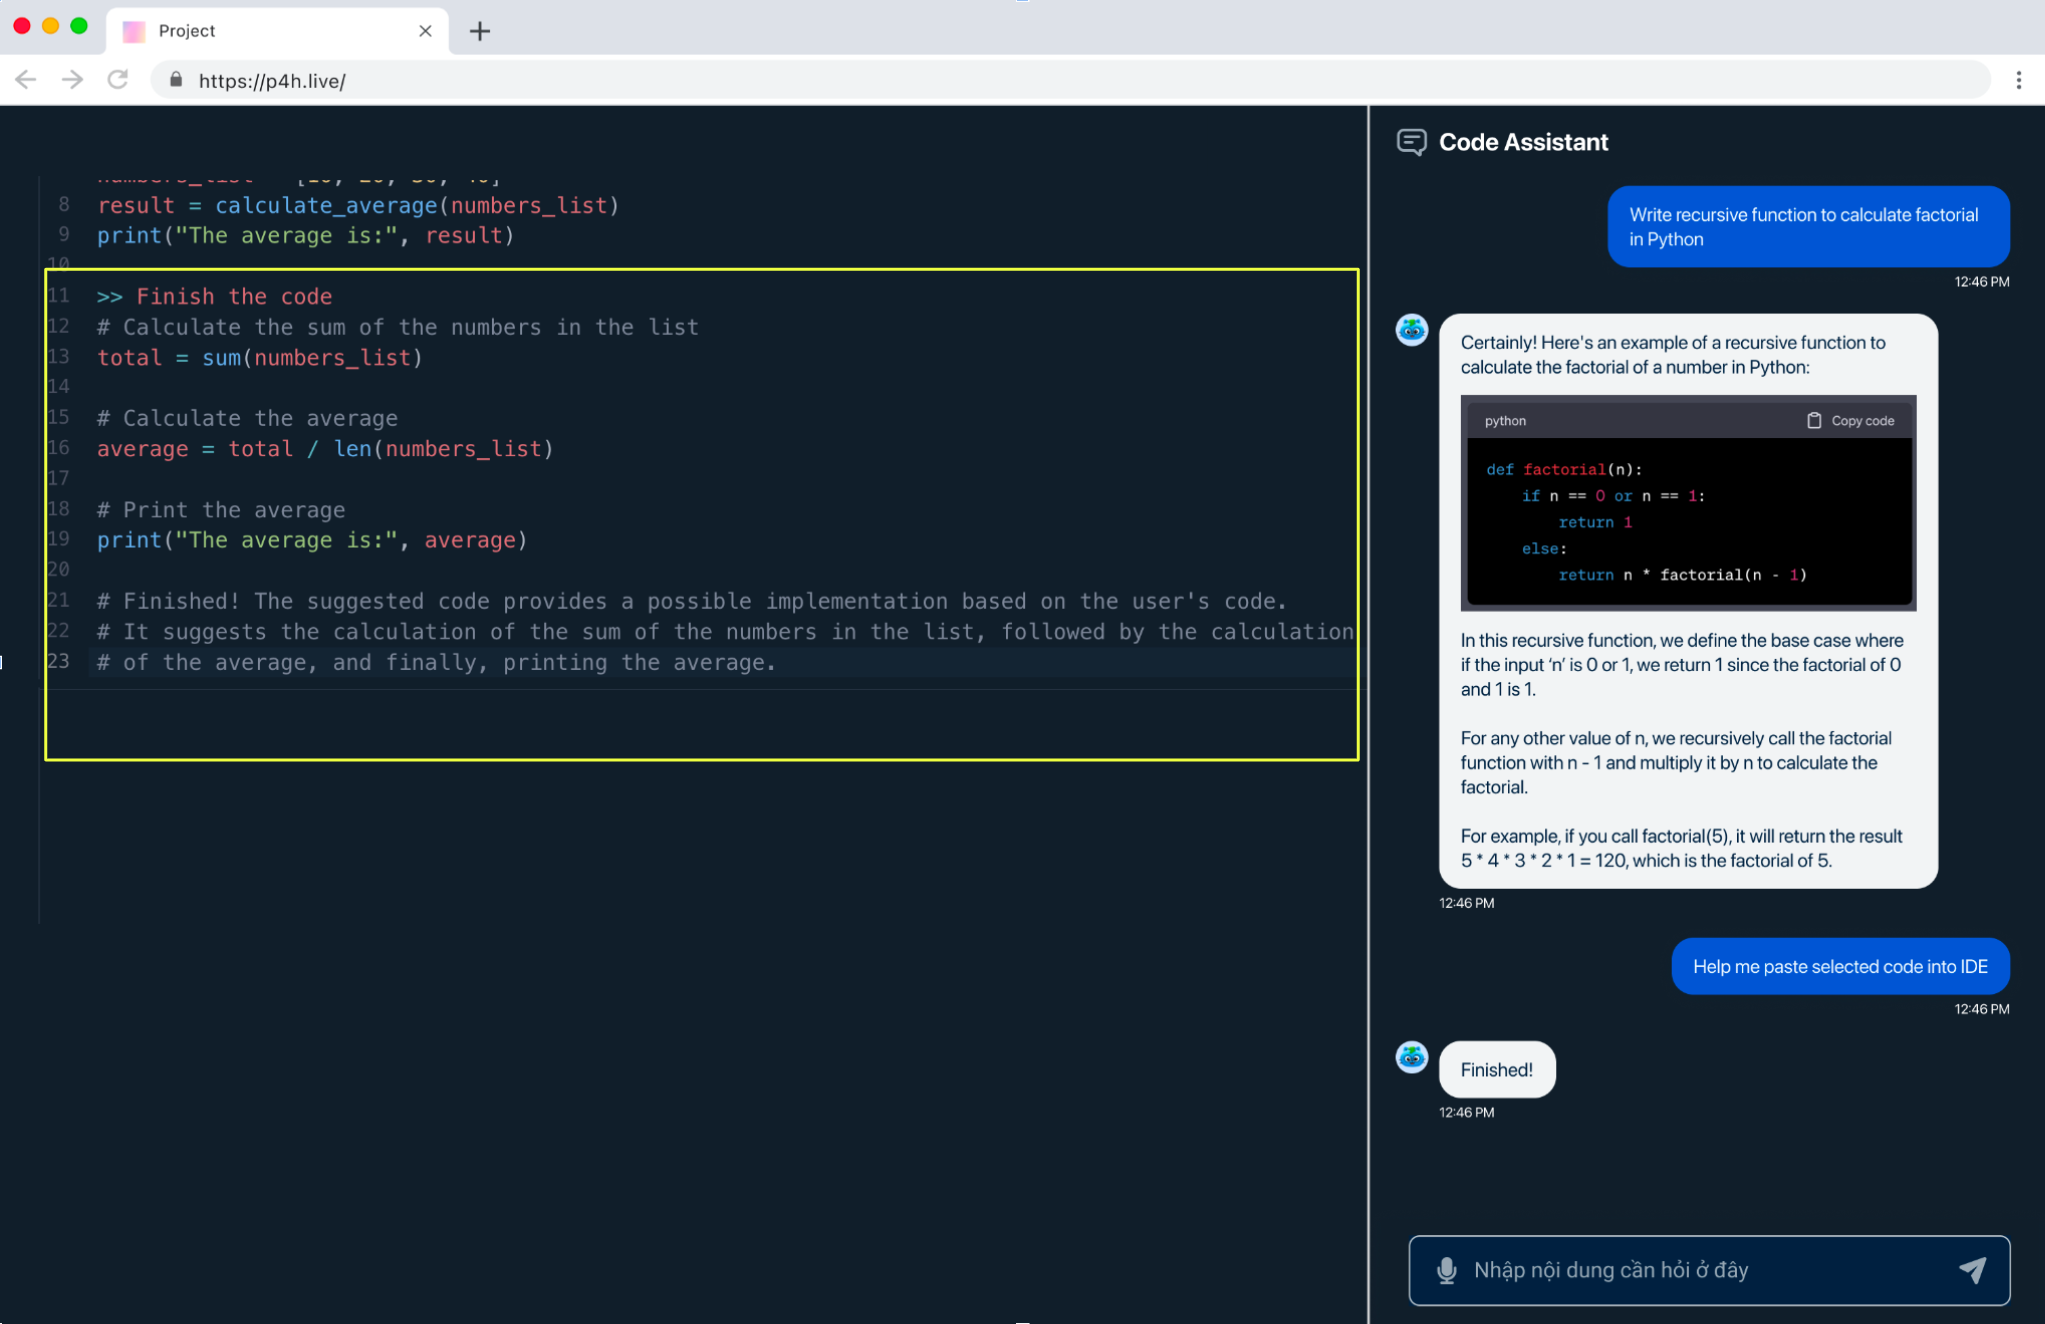
\includegraphics[width=.98\textwidth]{p4h-4}
%\end{minipage}  
%\caption{In-line Voice to Code Generation}
%\label{thrust3-two}
%\end{figure}

\noindent {\bf Voice for a Programming Task.} Sarah begins her coding
session by launching our proposed environment using voice
commands. The platform instantly activates, and she hears a
synthesized voice welcoming her.

{\em Setting Up the First Task: Computing Factorials and Storing in a
  List:} Sarah instructs the environment using natural language voice
commands, "I want to compute the factorial values of numbers from 1 to
100 and store those values in a list."

{\em Voice-to-Code Conversion - First Part:} The environment's
advanced voice recognition technology processes her command and
generates the initial code structure. Sarah continues to articulate
her requirements verbally, "For each number from 1 to 100, calculate
its factorial and add it to the factorial$\_$list."

{\em Real-time Code Generation}:
The environment translates her voice command into code (Figure~\ref{thrust3-one}).

{\em Verification and Documentation - First Part}: The environment
reads back the generated code to Sarah using synthesized speech. She
listens carefully to ensure that her intent is accurately translated
into code. Satisfied, she decides to generate comprehensive
documentation for this part of her code.

%{\em Integration and Test Cases - First Part:} Impressed with the
%environment's capabilities, Sarah seamlessly integrates her newly
%created code into her existing project, which focuses on mathematical
%computations. She also uses voice commands to create test cases for
%this part of her code.

{\em Requesting the Second Piece of Code: Computing Summation:} Having
successfully completed the first part of her task, Sarah now wants to
compute the summation of the factorial values stored in
factorial$\_$list. She issues a voice command to request the environment
to generate the code for this part of her task.

{\em Voice-to-Code Conversion - Second Part:} The environment
processes her new command and generates the code structure for
computing the summation.
Sarah continues with her voice commands, "Now, calculate the summation
of values in the factorial$\_$list and store it in total$\_$sum."

{\em Real-time Code Generation - Second Part:}
The environment translates her voice command into code.

{\em Verification and Documentation - Second Part:} The environment
reads back the generated code for the summation part. Sarah listens
carefully to ensure accuracy and completeness. Satisfied with the
code, she decides to generate comprehensive documentation for this
part as well.

%{\em Integration and Test Cases - Second Part:} Sarah integrates the
%newly generated code for summation into her existing project, ensuring
%that her project now computes and stores both the factorial values and
%their summation. She also creates test cases for this part of her
%code.

%With the help of this innovative programming environment, Sarah successfully completes her task. She feels empowered, as this environment not only mitigated accessibility barriers but also provided her with a versatile and inclusive toolset for a productive coding journey.

%==================================================


\begin{figure}[t]
\centering
\begin{minipage}{.48\textwidth}
%\begin{figure}[t]
\centering
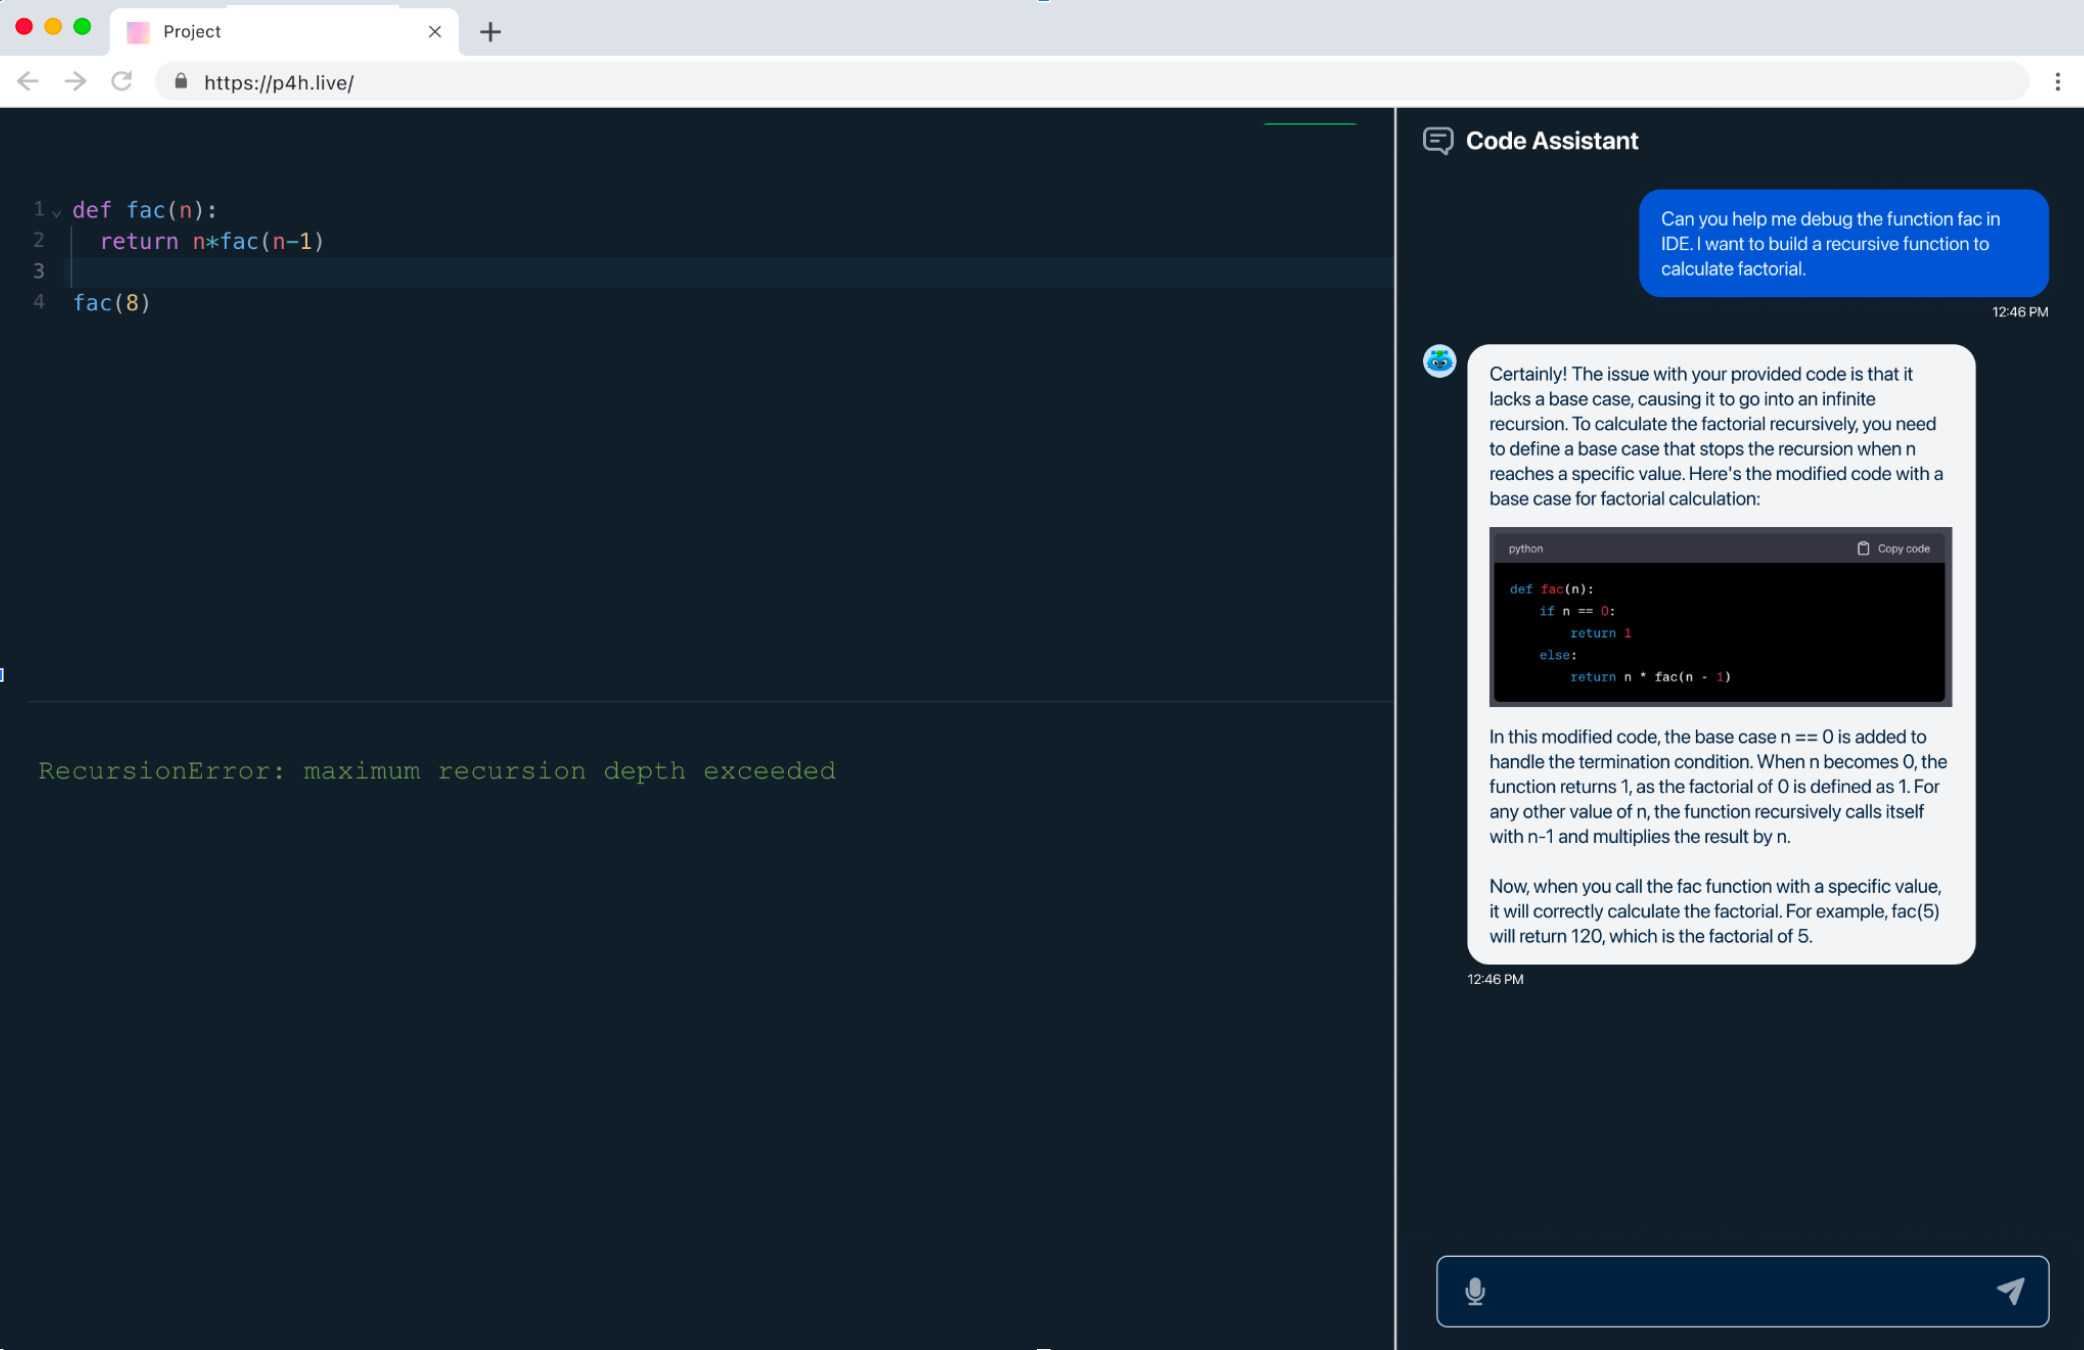
\includegraphics[width=.98\textwidth]{p4h-5}
%\caption{caption 1}
%\label{fig:left}
%\end{figure}
\end{minipage}
\begin{minipage}{.48\textwidth}
%\begin{figure}[t]
\centering
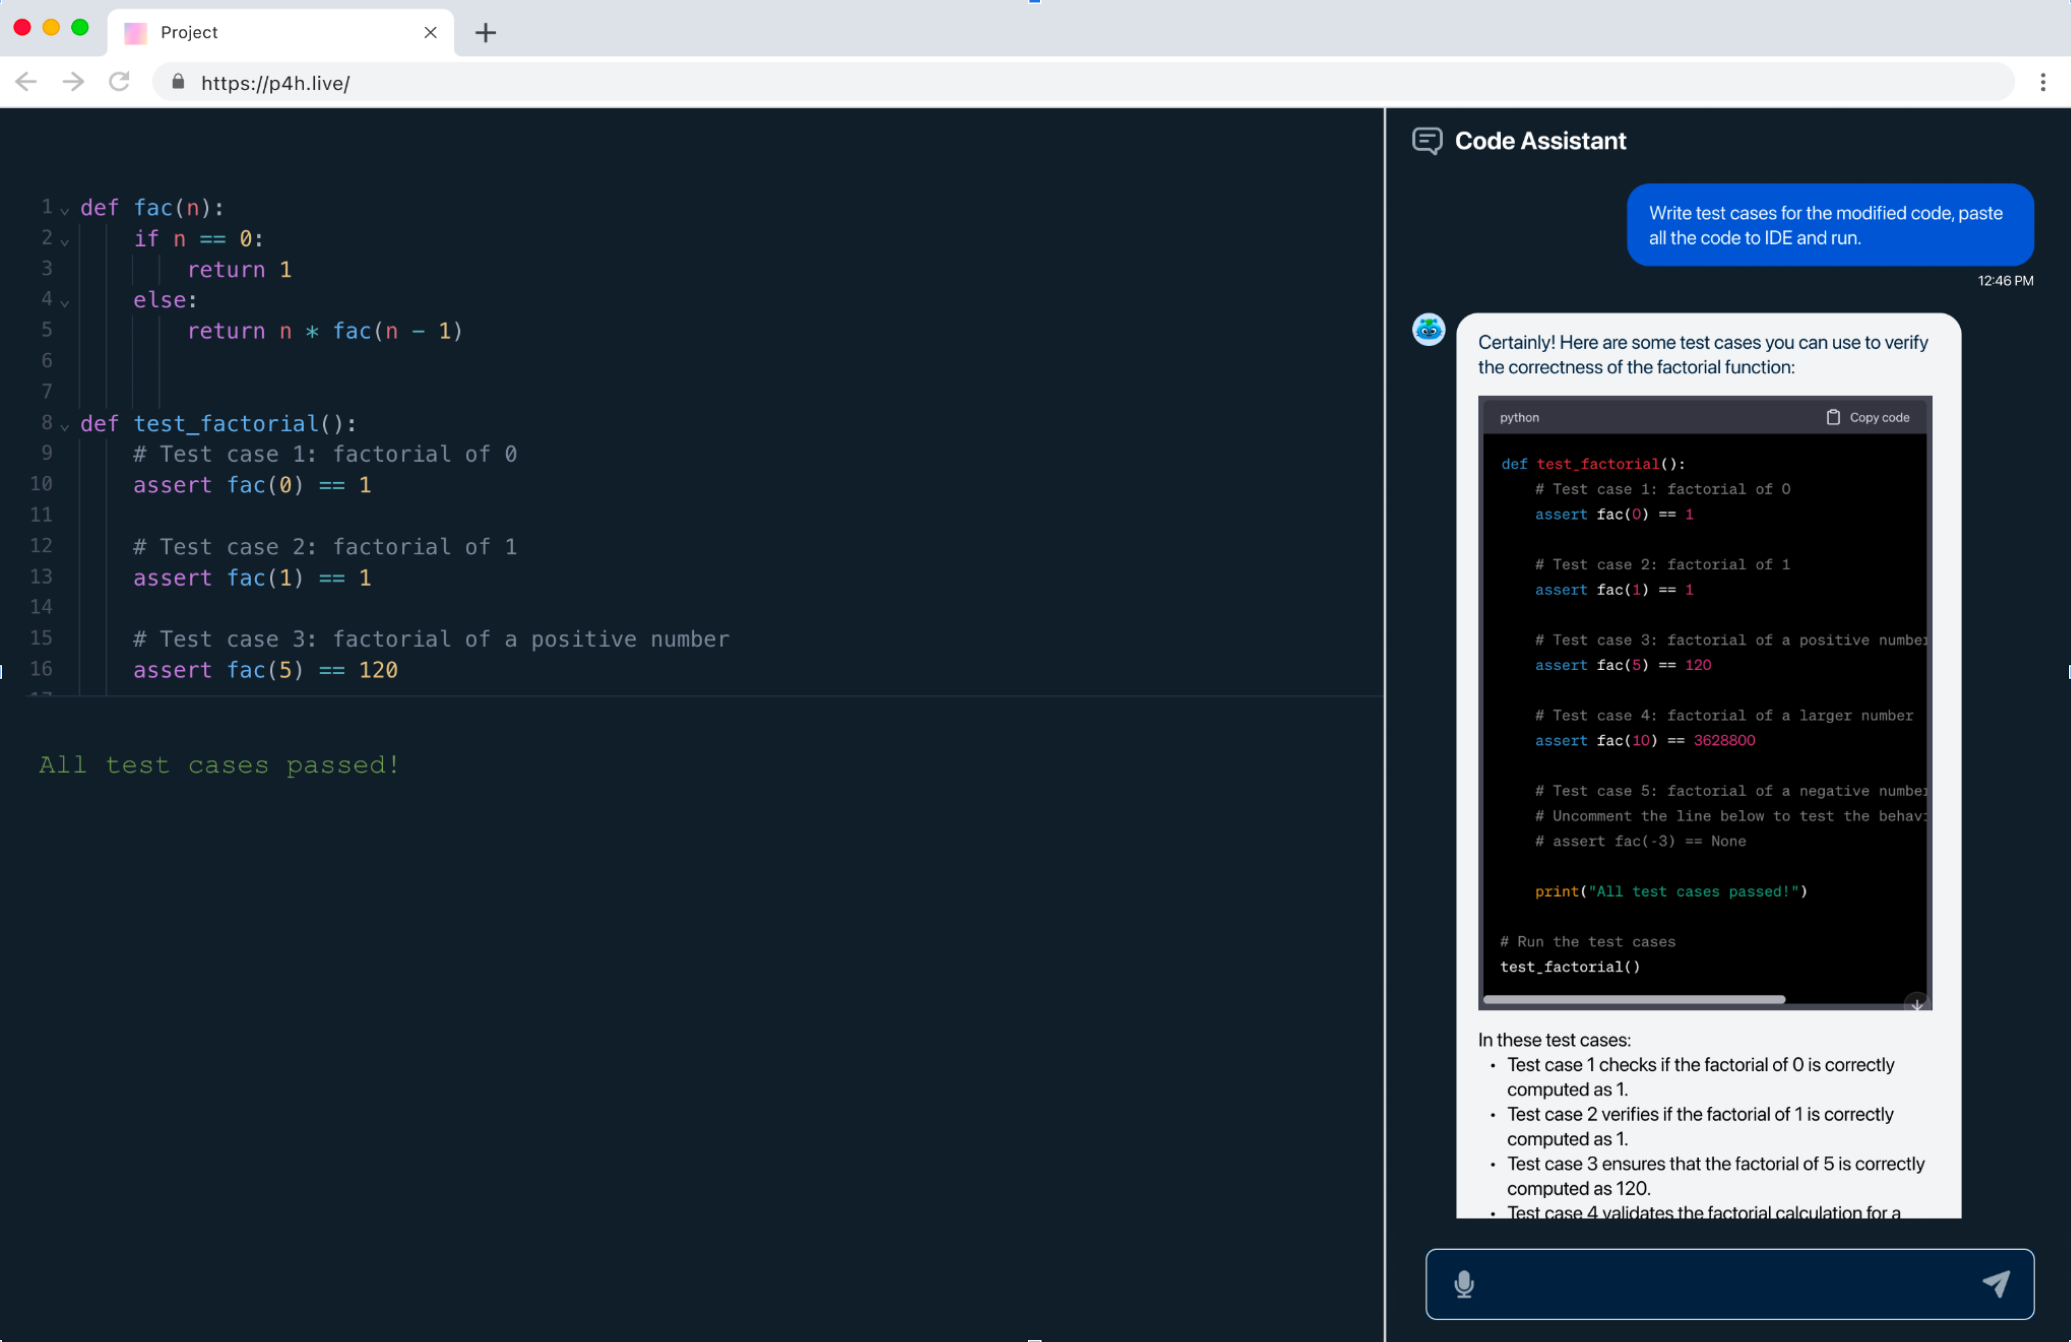
\includegraphics[width=.98\textwidth]{p4h-6}
%\caption{caption 2}
%\label{fig:right}
%\end{figure}
\end{minipage}  
%\vspace{-18pt}
\caption{Interactive, Voice-driven Debugging and Test Case Generation}
\label{thrust3-three}
\end{figure}

\noindent {\bf Interactive, Voice-driven Debugging and Test Case
  Generation.} In this use case scenario, a visually-impaired
programmer uses the programming environment to debug a buggy program
that calculates factorial values. They interact with the environment
using voice commands to pinpoint values at several statements and
finally identify the buggy statement.

{\em Initialization}: The visually-impaired programmer starts the
programming environment by saying, "Hey, Environment, open my
factorial program for debugging."  Voice Interaction: The environment
responds with a synthesized voice, "Your factorial program is open for
debugging. How can I assist you?"

{\em Setting Breakpoints and Value Request}: The programmer begins by
setting breakpoints at specific lines where they suspect issues. They
say, "Set a breakpoint at line 4 and another at line 7." The
programmer needs to inspect the values of variables at these
breakpoints. They ask, "What's the value of 'n' at line 4?"

{\em Environment Calls ChatGPT:} The programming environment
communicates with ChatGPT to fetch the value of 'n' at line 4.
ChatGPT generates the response: "The value of 'n' at line 4 is 5."

%\begin{wrapfigure}{r}{3.5in}
%\centering
%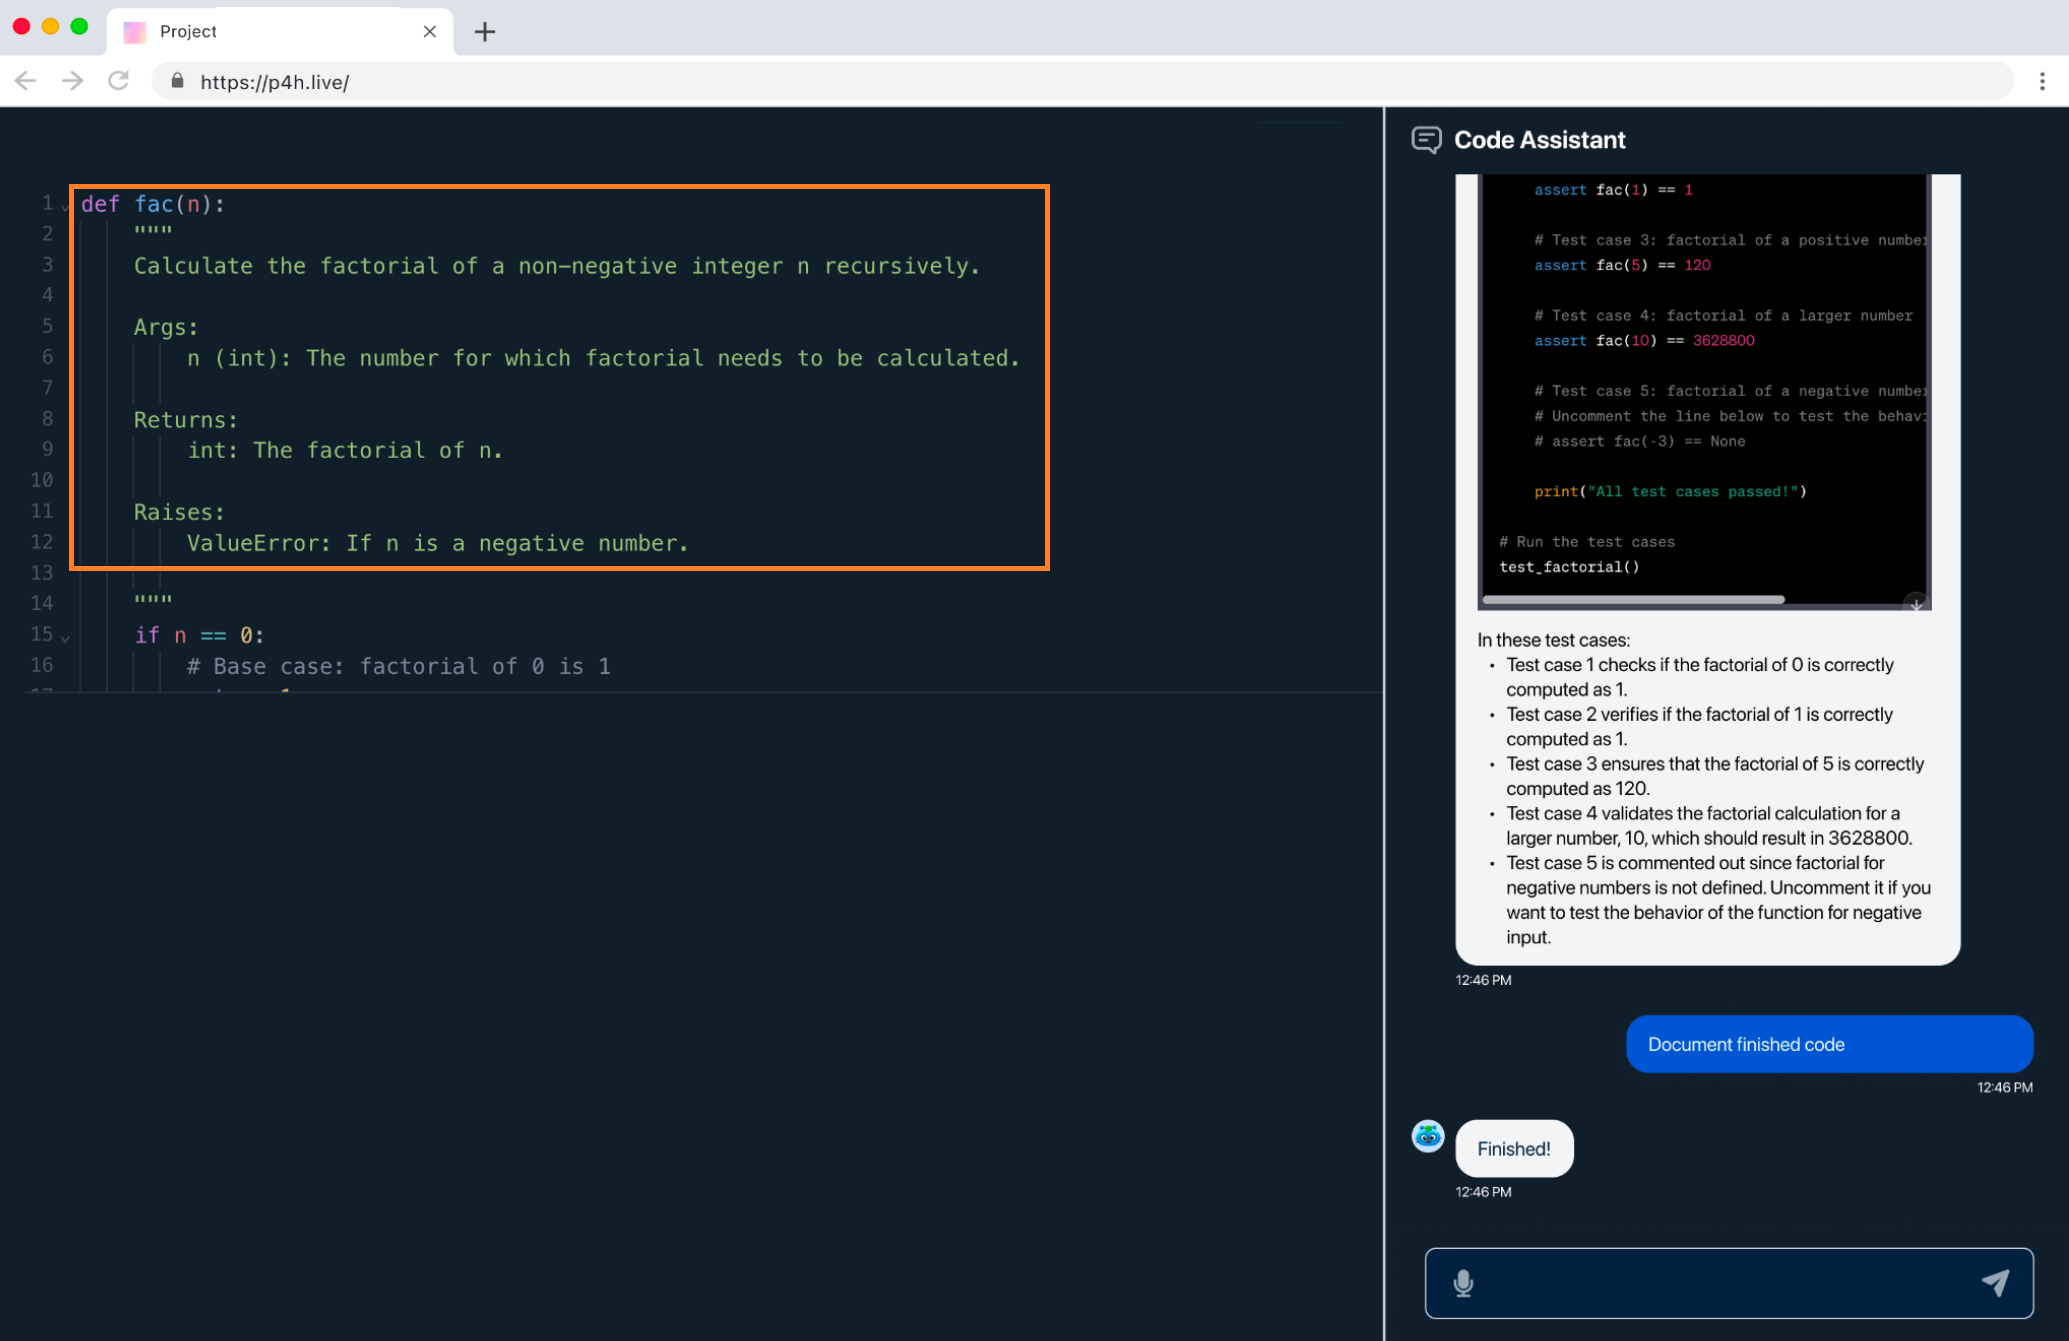
\includegraphics[width=3.4in]{p4h-7}
%\vspace{-6pt}
%\caption{Automated Documentation}
%\label{auto-doc}
%\end{wrapfigure}

{\em Verification and Iteration}: The programmer confirms the value of
'n' and continues, "What's the value of 'result' at line 7?"  The
environment again calls ChatGPT to obtain the value of 'result' at
line 7.
%It generates the response: "The value of 'result' at
%line 7 is~1."

{\em Pinpointing the Issue}: The programmer realizes that the value of
'result' should not be 1 at this point in the program. They suspect
there's an issue with the logic.  They ask, "What's the value of 'n'
at line 7?"  Environment Calls ChatGPT: The environment contacts
ChatGPT to retrieve the value of 'n' at line 7. It generates the
response: "The value of 'n' at line 7 is 4."

{\em Identifying and fixing the Bug}: The programmer now understands
that the value of 'result' is incorrect because 'n' should have been 4
at this point. They identify the buggy statement: "Looks like the
issue is at line 7. The recursive call should use 'n' minus 1."  (S)he
asks the environment to make the necessary correction, "Replace 'n -
1' with 'n' in the recursive call at line 7." The environment updates
the code.

{\em Testing Again:} The programmer decides to test the program: "Calculate the factorial of 5."  Code Execution: The
environment executes the corrected code and announces the result, "The
factorial of 5 is: 120."

{\bf Auto-generated Documentation and Comments.} In a scenario where a
VIPLs have just completed a coding project using our environment, they
utilize the power of voice interaction to request comprehensive
documentation for their code. With a simple voice command, they
instruct the environment to generate detailed documentation for their
project. The environment seamlessly responds by automatically creating
well-structured documentation, including explanations of functions,
variables, and comments.
%, all synthesized into an accessible format.

%This documentation not only serves as a valuable reference for the
%programmer but also enhances code accessibility and fosters
%collaboration with peers, ensuring that the visually-impaired
%programmer can fully document and share their work with colleagues.




%\begin{wrapfigure}{l}{0.5\textwidth}
%  \begin{center}
%    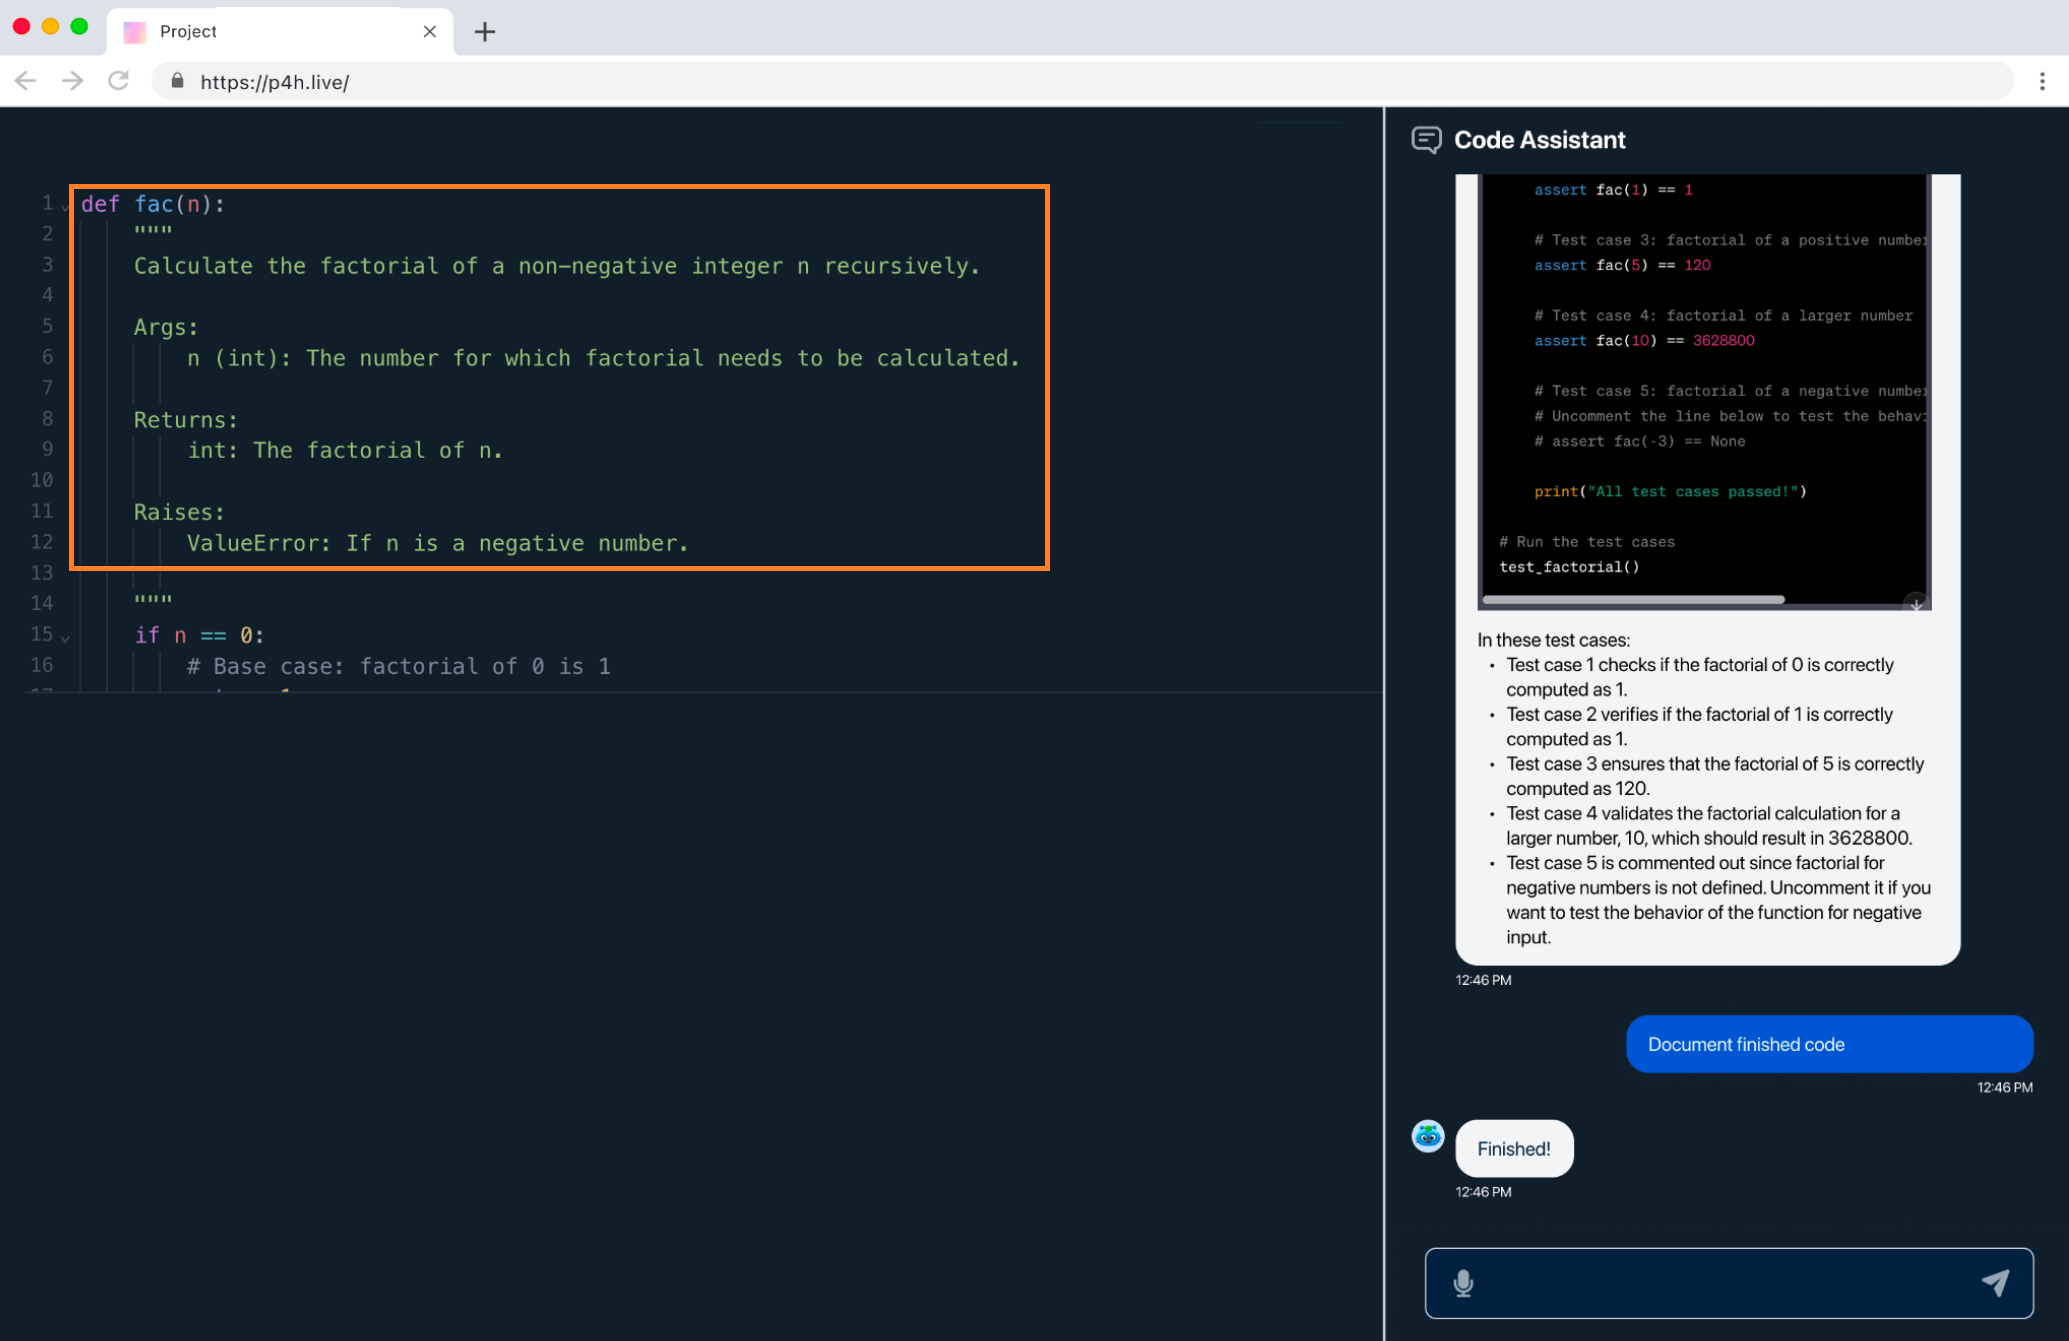
\includegraphics[width=3.2in]{p4h-7}
%  \end{center}
%  \vspace{-20pt}
%  \caption{Automated Documentation}
%\end{wrapfigure}



%Completion and Documentation:
%Satisfied with the result, the programmer can now complete the debugging process and document the changes made for future reference using voice commands.

%\begin{wrapfigure}{r}{0.625\textwidth}
%\vspace{-10pt}
%  \centering
%  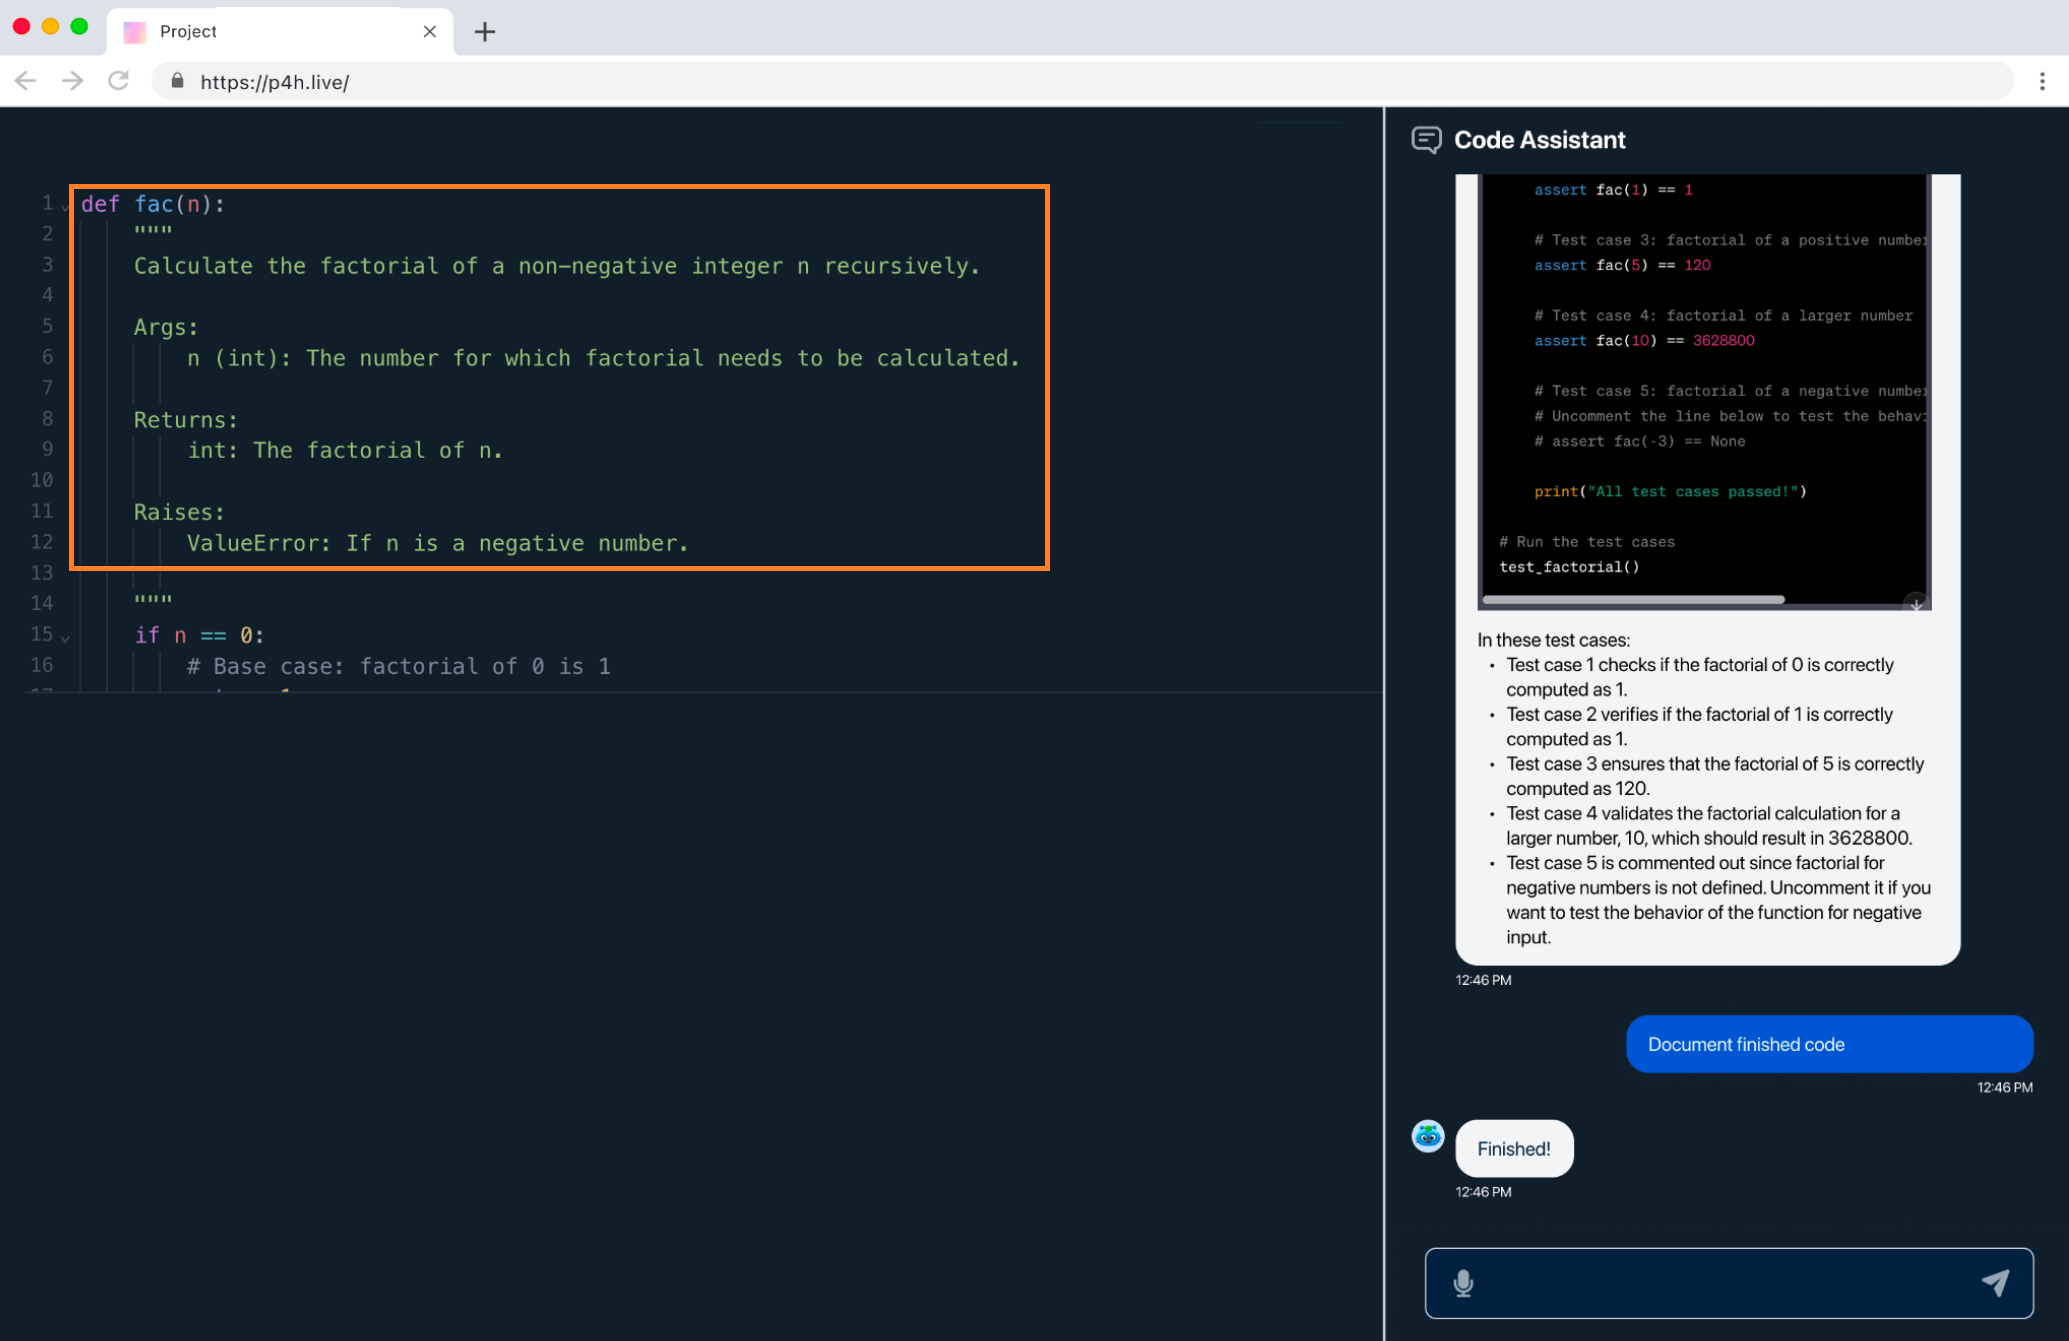
\includegraphics[width=3.2in]{p4h-7}
%\end{wrapfigure}
